\documentclass[a4paper,12pt]{article}

\usepackage{array}
\usepackage{graphicx}
\usepackage{color}
\usepackage{colortbl}
\usepackage[export]{adjustbox}
\usepackage{multirow}
\usepackage{ctable}

\usepackage{geometry}
 \geometry{
 a4paper,
 total={210mm,297mm},
 left=20mm,
 right=20mm,
 top=16mm,
 bottom=15mm,
 }

\definecolor{lowgray}{rgb}{0.8,0.8,0.8}
\definecolor{gray2}{rgb}{0.6,0.6,0.6}

\newcolumntype{L}[1]{>{\raggedright\let\newline\\\arraybackslash\hspace{0pt}}m{#1}}
\newcolumntype{C}[1]{>{\centering\let\newline\\\arraybackslash\hspace{0pt}}m{#1}}
\newcolumntype{R}[1]{>{\raggedleft\let\newline\\\arraybackslash\hspace{0pt}}m{#1}}

\newlength{\Oldarrayrulewidth}
\newcommand{\ClineProto}[2]{%
  \noalign{\global\setlength{\Oldarrayrulewidth}{\arrayrulewidth}}%
  \noalign{\global\setlength{\arrayrulewidth}{#1}}\cline{#2}%
  \noalign{\global\setlength{\arrayrulewidth}{\Oldarrayrulewidth}}}
\newcommand{\Cline}[2]{\arrayrulecolor{lowgray}\ClineProto{#1}{#2}\arrayrulecolor{black}}

\newcommand\VRule[1][\arrayrulewidth]{\vrule width #1}

\title{\textbf{CURRICULUM VITAE}}
\date{\vspace{0ex}}

\begin{document}

\maketitle

%\setlength{\arrayrulewidth}{0.05pt}
% \setlength{\extrarowheight}{20pt}
\begin{tabular}{| L{12.75cm} !{\color{lowgray}\VRule[0.001pt]} C{3.1cm} |}
\hline
\rowcolor{lowgray}
\multicolumn{2}{|c|}{ }\\[-0.42cm]
\rowcolor{lowgray}
\multicolumn{2}{|c|}{\textbf{PERSONAL INFORMATION}}\\
\hline
Full name: NGUYEN NGOC SON & \multirow{6}{3.5cm}{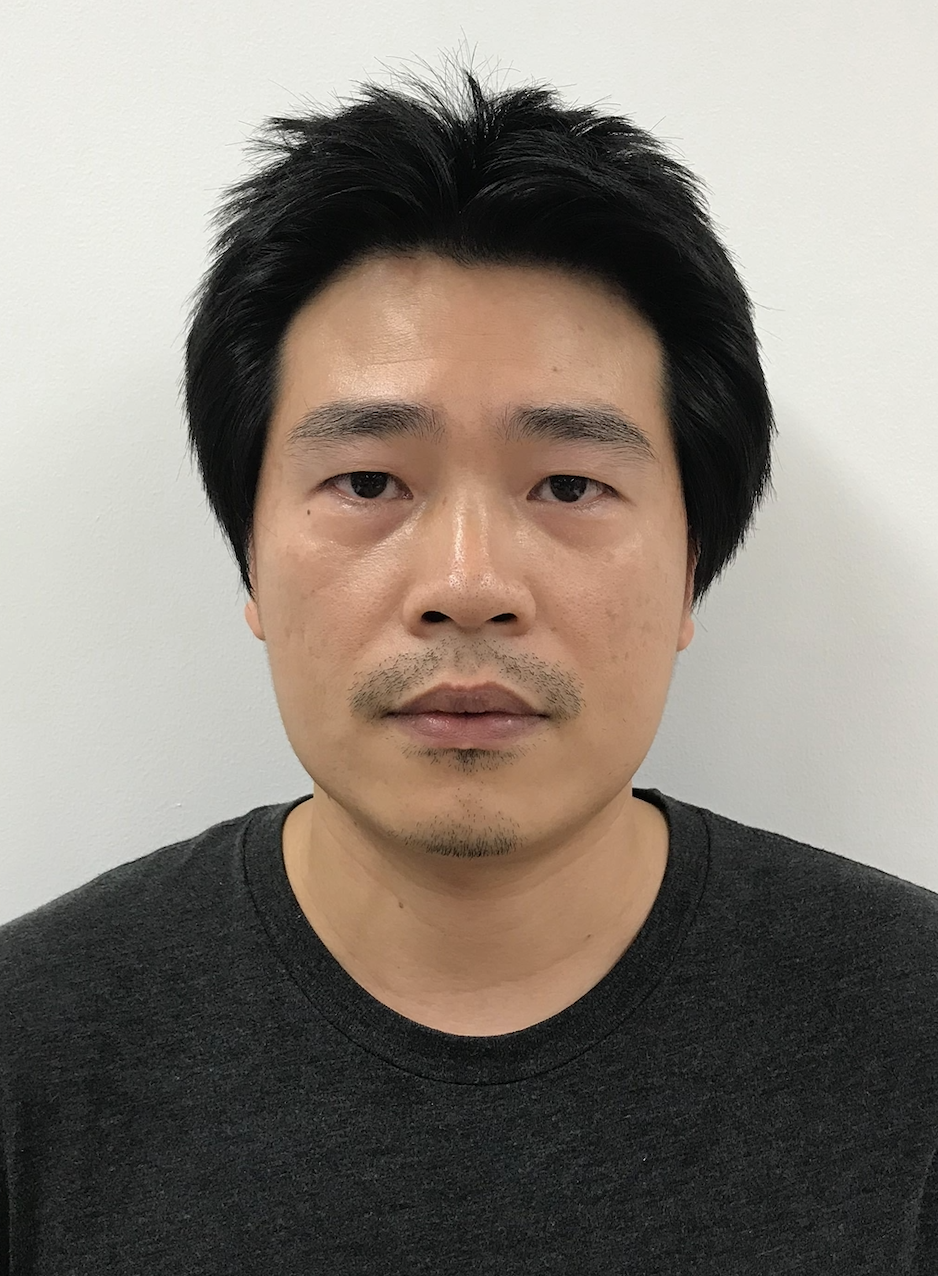
\includegraphics[trim=0.2cm 0.1cm 0.2cm 0.65cm, width=3.1cm, height=4.1cm]{portrait.png}} \\
\Cline{0.005pt}{1-1}
&\\[-0.35cm]
Gender: Male & \\[0.1cm]
\Cline{0.005pt}{1-1}
&\\[-0.35cm]
Nationality: Vietnam & \\[0.1cm]
\Cline{0.005pt}{1-1}
&\\[-0.35cm]
Date of birth: June 26, 1985 & \\[0.1cm]
\Cline{0.005pt}{1-1}
&\\[-0.35cm]
Address: No. 101, Grand Mere Noborito, Noborito 3276, Tama-ku, Kawasaki-shi, Kanagawa-ken, 214-0014 Japan & \\[0.35cm]
\Cline{0.005pt}{1-1}
&\\[-0.35cm]
Email: ngocson2vn@gmail.com & \\[0.1cm]
Mobile: 080-5228-5269 & \\[0.1cm]
\hline
\end{tabular}
\\[1.0cm]

\begin{tabular}{| L{16.268cm} |}
\hline
\rowcolor{lowgray}
\multicolumn{1}{|c|}{ }\\[-0.42cm]
\rowcolor{lowgray}
\multicolumn{1}{|c|}{\textbf{PROFESSIONAL SUMMARY}} \\
\hline
\\[-0.3cm]
\quad After graduating from university, the first software company I joined is USOL Vietnam, an offshore company of Nihon Unisys Japan. Here, I participated in a software development process including Designing, Developing, and Testing for e-commerce systems, banking systems, and CRM systems for Japanese customers. I was involved in a very big software project of reconstructing the core e-commerce system of Nissen Japan. Therefore, I obtained a lot of experience in Software Development. \\
\\[-0.3cm]
\quad After that, I switched to the field of Game Engineering. I worked as a Game Engineer for Punch Entertainment Vietnam for a short period. Then, Punch Entertainment Vietnam joined DeNA Japan, it became DeNA Hanoi, a subsidiary of DeNA Japan. At DeNA Hanoi, I worked as an IT Infrastructure Engineer. My primary responsibility was to keep DeNA's services fast and stable. Daily, I cooperated with Japanese Engineers in Tokyo to build and operate game server systems for World Wide, Japan, Korea, China, and Taiwan markets on Amazon Web Services. \\
\\[-0.3cm]
\quad Since 2014, I have relocated to Japan and started a new chapter in my life here. At the beginning, I was working as a Part-time Research Collaborator at Earthquake Engineering Laboratory, College of Engineering, Nihon University. I collaborated with professor Susumu Nakamura on developing a computational simulation software using Material Point Method for
simulating and predicting landslide phenomena.\\
\\[-0.3cm]
\quad Since 2017, I have joined a health-care startup named FiNC Technologies in Tokyo and I have worked as a Site Reliability Engineer (SRE). I was responsible for building and operating the IT infrastructure environment for FiNC app on Amazon Web Services (AWS). Recently, I have taken on the Data Engineer position and I have been responsible for building and maintaining a Big Data Platform for FiNC Technologies.\\[1.3cm]
\hline
\end{tabular}
\\[1.0cm]

% ===========================================================================================================
% \newpage

\begin{tabular}{| L{6.5cm} !{\color{lowgray}\VRule[0.001pt]} L{4.3cm} !{\color{lowgray}\VRule[0.001pt]} L{2.7cm} !{\color{lowgray}\VRule[0.001pt]} L{1.5cm} |}
\hline
\rowcolor{lowgray}
\multicolumn{4}{|c|}{ }\\[-0.42cm]
\rowcolor{lowgray}
\multicolumn{4}{|c|}{\textbf{EDUCATION}} \\
\hline
%\\[-0.3cm]
\textbf{University} & \textbf{Faculty} & \textbf{Graduation year} & \textbf{Grade} \\
\Cline{0.005pt}{1-4}
Vietnam National University, Hanoi College of Science & Mathematics--Mechanics--Informatics & 2007 & Good \\
\hline
\end{tabular}
\\[1.0cm]

\begin{tabular}{| L{16.268cm} |}
\hline
\rowcolor{lowgray}
\multicolumn{1}{|c|}{ }\\[-0.42cm]
\rowcolor{lowgray}
\multicolumn{1}{|c|}{\textbf{HONORS AND AWARDS}} \\
\hline
\\[-0.3cm]
Awarded 2005 Toyota Scholarship -- Toyota Vietnam Foundation \\[0.15cm]
\hline
\end{tabular}
\\[1.0cm]

\begin{tabular}{| L{16.268cm} |}
\hline
\rowcolor{lowgray}
\multicolumn{1}{|c|}{ }\\[-0.42cm]
\rowcolor{lowgray}
\multicolumn{1}{|c|}{\textbf{LICENSES AND CERTIFICATIONS}} \\
\hline
\\[-0.15cm]
Certificate: \textbf{AWS Certified Solutions Architect - Professional} \\
Issuer: Amazon Web Services, Inc. \\
Issue date: September 13, 2019 \\
Expiration date: September 13, 2022 \\
Validation number: G7Q7XHV1GMBQQSSF \\
Validate at: http://aws.amazon.com/verification \\

\\[-0.1cm]
\Cline{0.005pt}{1-1}
\\[-0.1cm]

Certificate: \textbf{AWS Certified Security - Specialty} \\
Issuer: Amazon Web Services, Inc. \\
Issue date: October 15, 2019 \\
Expiration date: October 15, 2022 \\
Validation number: 064TLSWCGNB118WL \\
Validate at: http://aws.amazon.com/verification \\[0.15cm]
\hline
\end{tabular}
\\[1.0cm]

\begin{tabular}{| L{5.5cm} !{\color{lowgray}\VRule[0.001pt]} L{10.348cm} |}
\hline
\rowcolor{lowgray}
\multicolumn{2}{|c|}{ }\\[-0.42cm]
\rowcolor{lowgray}
\multicolumn{2}{|c|}{\textbf{LANGUAGE}} \\
\hline
& \\[-0.3cm]
\textbf{Language} & \textbf{Proficiency} \\[0.15cm]
\Cline{0.005pt}{1-2}
 & \\[-0.3cm]
Vietnamese & Native level \\[0.15cm]
\Cline{0.005pt}{1-2}
 & \\[-0.3cm]
English & Business level \\[0.15cm]
\Cline{0.005pt}{1-2}
 & \\[-0.3cm]
Japanese & Equivalent to JLPT N2 \\[0.15cm]
\hline
\end{tabular}
\\[1.0cm]


% ===========================================================================================================
\newpage

\begin{tabular}{| L{6.6cm} !{\color{lowgray}\VRule[0.001pt]} L{5cm} !{\color{lowgray}\VRule[0.001pt]} L{4cm} |}

\hline
\rowcolor{lowgray}
\multicolumn{3}{|c|}{ }\\[-0.42cm]
\rowcolor{lowgray}
\multicolumn{3}{|C{16.27cm}|}{\textbf{EXPERIENCE}} \\
\hline

\end{tabular}
\\[0.2cm]

\begin{tabular}{| L{6.42cm} !{\color{lowgray}\VRule[0.001pt]} L{5cm} !{\color{lowgray}\VRule[0.001pt]} L{4cm} |}

\hline
\multicolumn{3}{|l|}{} \\[-0.35cm]
\multicolumn{3}{|l|}{\textbf{Company: FiNC, Inc.}} \\[0.1cm]
\hline
& & \\[-0.4cm]
Position: SRE Engineer & From: February 2017 & To: February 2020 \\[0.1cm]
\Cline{0.005pt}{1-3}

\multicolumn{3}{|l|}{} \\[-0.2cm]
\multicolumn{3}{|l|}{Responsibilities:} \\
\multicolumn{3}{|l|}{\quad- Building infrastructure for Microservices.} \\
\multicolumn{3}{|l|}{\quad- Keeping FiNC services fast and reliable.} \\
\multicolumn{3}{|l|}{} \\[-0.2cm]

\multicolumn{3}{|l|}{Technologies:} \\
\multicolumn{3}{|l|}{\quad- Amazon Web Services: ECS, Batch, Lambda, RDS, Route53, S3, etc} \\
\multicolumn{3}{|l|}{\quad- Jenkins} \\[0.2cm]
\multicolumn{3}{|l|}{\quad- New Relic, Datadog, Zabbix} \\[0.2cm]
\multicolumn{3}{|l|}{\quad- Golang, Python, Ruby, NodeJS} \\[0.2cm]
\hline

\end{tabular}
\\[0.5cm]

\begin{tabular}{| L{7.82cm} !{\color{lowgray}\VRule[0.001pt]} L{4cm} !{\color{lowgray}\VRule[0.001pt]} L{3.6cm} |}

\hline
\multicolumn{3}{|l|}{} \\[-0.35cm]
\multicolumn{3}{|l|}{\textbf{Company: Nihon University, College of Engineering}} \\[0.1cm]
\hline
& & \\[-0.4cm]
Position: Part-time Research Collaborator & From: October 2014 & To: March 2016 \\[0.1cm]
\Cline{0.005pt}{1-3}

\multicolumn{3}{|l|}{} \\[-0.2cm]
\multicolumn{3}{|l|}{Responsibilities:} \\
\multicolumn{3}{|L{15cm}|}{\quad- Developing a computational simulation software based on Material Point Method for simulating and predicting landslide phenomena.} \\
\multicolumn{3}{|l|}{} \\[-0.2cm]

\multicolumn{3}{|l|}{Technologies:} \\
\multicolumn{3}{|l|}{\quad- Fortran 90} \\
\multicolumn{3}{|l|}{\quad- MPI Parallel Programming} \\[0.2cm]
\hline

\end{tabular}
\\[0.5cm]

\begin{tabular}{| L{7.82cm} !{\color{lowgray}\VRule[0.001pt]} L{4cm} !{\color{lowgray}\VRule[0.001pt]} L{3.6cm} |}

\hline
\multicolumn{3}{|l|}{} \\[-0.35cm]
\multicolumn{3}{|l|}{\textbf{Company: DeNA Hanoi, subsidiary of DeNA Japan}} \\[0.1cm]
\hline
& & \\[-0.4cm]
Position: IT Infrastructure Engineer & From: December 2011 & To: January 2014 \\[0.1cm]
\Cline{0.005pt}{1-3}

\multicolumn{3}{|l|}{} \\[-0.2cm]
\multicolumn{3}{|l|}{Responsibilities:} \\
\multicolumn{3}{|L{15cm}|}{\quad- Cooperating with Japanese Engineers in Tokyo to operate game servers for World Wide, Japan, Korea, China and Taiwan markets on mobage social network.} \\
\multicolumn{3}{|L{15cm}|}{\quad- Building infrastructure for games on Amazon Web Services, using EC2, VPC, S3, Route53 and CloudWatch services.} \\
\multicolumn{3}{|L{15cm}|}{\quad- Support Game Engineers to investigate game errors.} \\
\multicolumn{3}{|L{15cm}|}{\quad- Monitoring more than 200 servers 24/7, estimating servers workload and scaling servers.} \\
\multicolumn{3}{|L{15cm}|}{\quad- Studying and developing operation tools.} \\
\multicolumn{3}{|L{15cm}|}{\quad- Managing Firewall, Router and Switch in company network.} \\
\multicolumn{3}{|l|}{} \\[-0.2cm]

\multicolumn{3}{|l|}{Technologies:} \\
\multicolumn{3}{|l|}{\quad- Amazon Web Services} \\
\multicolumn{3}{|l|}{\quad- Linux, Apache, Nginx, Perl and PHP} \\
\multicolumn{3}{|l|}{\quad- NodeJS} \\
\multicolumn{3}{|l|}{\quad- MySQL, MHA, MyDNS} \\
\multicolumn{3}{|l|}{\quad- qmail} \\
\multicolumn{3}{|l|}{\quad- Monitoring tools: Nagios, Cacti, CloudForecast, GrowthForecast, Perl scripts} \\
\multicolumn{3}{|l|}{\quad- Cisco IOS, Juniper ScreenOS} \\[0.2cm]
\hline

\end{tabular}
\\[0.5cm]

\begin{tabular}{| L{7.82cm} !{\color{lowgray}\VRule[0.001pt]} L{4cm} !{\color{lowgray}\VRule[0.001pt]} L{3.6cm} |}

\hline
\multicolumn{3}{|l|}{} \\[-0.35cm]
\multicolumn{3}{|l|}{\textbf{Company: Punch Entertainment Vietnam}} \\[0.1cm]
\hline
& & \\[-0.4cm]
Position: Game Engineer & From: May 2011 & To: December 2011 \\[0.1cm]
\Cline{0.005pt}{1-3}

\multicolumn{3}{|l|}{} \\[-0.2cm]
\multicolumn{3}{|l|}{Responsibilities:} \\
\multicolumn{3}{|l|}{\quad- Developing web games on \textbf{facebook}.} \\
\multicolumn{3}{|L{15cm}|}{\quad- Developing Android and iOS games (client and server sides) on \textbf{mobage} social network.} \\
\multicolumn{3}{|l|}{\quad- Deploying and monitoring game servers on Amazon Web Services.} \\
\multicolumn{3}{|l|}{} \\[-0.2cm]

\multicolumn{3}{|l|}{Technologies:} \\
\multicolumn{3}{|l|}{\quad- ActionScript, SmartFox} \\
\multicolumn{3}{|l|}{\quad- Amazon Web Services} \\
\multicolumn{3}{|l|}{\quad- NodeJS} \\
\multicolumn{3}{|l|}{\quad- Perl} \\
\multicolumn{3}{|l|}{\quad- HTML, jQuery, Dojo, CSS} \\
\multicolumn{3}{|l|}{\quad- Java, SpringRoo, Hibernate FW} \\
\multicolumn{3}{|l|}{\quad- MySQL} \\[0.2cm]
\hline

\end{tabular}
\\[0.5cm]

\begin{tabular}{| L{7.82cm} !{\color{lowgray}\VRule[0.001pt]} L{4cm} !{\color{lowgray}\VRule[0.001pt]} L{3.6cm} |}

\hline
\multicolumn{3}{|l|}{} \\[-0.35cm]
\multicolumn{3}{|l|}{\textbf{Company: USOL Vietnam, an offshore company of Nihon Unisys Japan}} \\[0.1cm]
\hline
& & \\[-0.4cm]
Position: Software Developer & From: June 2008 & To: April 2011 \\[0.1cm]
\Cline{0.005pt}{1-3}

\multicolumn{3}{|l|}{} \\[-0.2cm]
\multicolumn{3}{|l|}{Responsibilities:} \\
\multicolumn{3}{|L{15cm}|}{\quad- Participating in software development process including Designing, Developing and Testing for shopping systems, banking systems, CRM systems of Japanese customers.} \\
\multicolumn{3}{|L{15cm}|}{\quad- Participating in software projects associated with big customers in Japan such as Nissen, JETRO - Japan External Trade Organization.} \\
\multicolumn{3}{|l|}{} \\[-0.2cm]

\multicolumn{3}{|l|}{Technologies:} \\
\multicolumn{3}{|l|}{\quad- ASP.NET, ADO.NET, C\#.NET} \\
\multicolumn{3}{|l|}{\quad- Java EE, Struts, Spring, Hibernate frameworks} \\
\multicolumn{3}{|l|}{\quad- HTML, jQuery, CSS} \\
\multicolumn{3}{|l|}{\quad- SQL Server, Oracle Server} \\[0.1cm]
\hline

\end{tabular}
\\[0.5cm]

\begin{tabular}{| L{7.82cm} !{\color{lowgray}\VRule[0.001pt]} L{4cm} !{\color{lowgray}\VRule[0.001pt]} L{3.6cm} |}

\hline
\multicolumn{3}{|l|}{} \\[-0.35cm]
\multicolumn{3}{|l|}{\textbf{Company: Vietnam Institute of Mechanics}} \\[0.1cm]
\hline
& & \\[-0.4cm]
Position: Researcher & From: July 2007 & To: November 2007 \\[0.1cm]
\Cline{0.005pt}{1-3}

\multicolumn{3}{|l|}{} \\[-0.2cm]
\multicolumn{3}{|l|}{Responsibilities:} \\
\multicolumn{3}{|l|}{\quad- Studying documents of oil well.} \\
\multicolumn{3}{|l|}{\quad- Developing computational programs for liquid laboratory.} \\
\multicolumn{3}{|l|}{} \\[-0.2cm]

\multicolumn{3}{|l|}{Technologies:} \\
\multicolumn{3}{|l|}{\quad- Fortran 90} \\[0.1cm]
\hline

\end{tabular}
\\[0.5cm]

\begin{tabular}{| L{7.82cm} !{\color{lowgray}\VRule[0.001pt]} L{4cm} !{\color{lowgray}\VRule[0.001pt]} L{3.6cm} |}

\hline
\multicolumn{3}{|l|}{} \\[-0.35cm]
\multicolumn{3}{|l|}{\textbf{Company: MED-AID VIET NAM}} \\[0.1cm]
\hline
& & \\[-0.4cm]
Position: Researcher & From: June 2005 & To: December 2005 \\[0.1cm]
\Cline{0.005pt}{1-3}

\multicolumn{3}{|l|}{} \\[-0.2cm]
\multicolumn{3}{|l|}{Responsibilities:} \\
\multicolumn{3}{|l|}{\quad- Studying scanner documents and reading source code of scanner system.} \\
\multicolumn{3}{|l|}{\quad- Proposing improvements in source code.} \\
\multicolumn{3}{|l|}{} \\[-0.2cm]

\multicolumn{3}{|l|}{Technologies:} \\
\multicolumn{3}{|l|}{\quad- Microsoft Visual C++} \\[0.1cm]
\hline

\end{tabular}


\begin{tabular}{| L{6.42cm} !{\color{lowgray}\VRule[0.001pt]} L{5cm} !{\color{lowgray}\VRule[0.001pt]} L{4cm} |}

\hline
\multicolumn{3}{|l|}{} \\[-0.35cm]
\multicolumn{3}{|l|}{\textbf{Company: Supervisor.org, an open source project}} \\[0.1cm]
\hline
& & \\[-0.4cm]
Position: Contributor & From: July 2014 & To: Now \\[0.1cm]
\Cline{0.005pt}{1-3}

\multicolumn{3}{|l|}{} \\[-0.2cm]
\multicolumn{3}{|l|}{Responsibilities:} \\
\multicolumn{3}{|L{15cm}|}{\quad- Developing a client/server system that allows its users to monitor and control a number of processes on UNIX-like operating systems.} \\
\multicolumn{3}{|l|}{} \\[-0.2cm]

\multicolumn{3}{|l|}{Technologies:} \\
\multicolumn{3}{|l|}{\quad- Python} \\[0.2cm]
\hline

\end{tabular}

\end{document}